\documentclass{article}
\usepackage{mathtext}
\usepackage[russian]{babel}
\usepackage[a4paper, top=2cm, bottom=2cm, left=0.9cm, right=0.9cm, marginparwidth=1.75cm]{geometry}
\usepackage{amsmath}
\usepackage{amssymb}
\usepackage{multicol}
\usepackage{fancyhdr}
\usepackage{nicefrac}
\usepackage{graphicx}
\usepackage{cancel}
\usepackage{wrapfig}
\usepackage{tikz}

\pagestyle{fancy}
\fancyhead[L]{Математический анализ (весна'23)}
\fancyhead[R]{Овчинников Павел, Румянцев Алексей, Чебаненко Дмитрий (1.6)}

\newlength{\tempheight}
\newcommand{\Let}[0]{%
\mathbin{\text{\settoheight{\tempheight}{\mathstrut}\raisebox{0.5\pgflinewidth}{%
\tikz[baseline,line cap=round,line join=round] \draw (0,0) --++ (0.4em,0) --++ (0,1.5ex) --++ (-0.4em,0);%
}}}\;}
\newcommand{\e}{\text{e}}
\newcommand{\la}{\lambda}
\newcommand{\shiftleft}[3]{\makebox[#1][r]{\makebox[#2][l]{#3}}}
\newcommand{\shiftright}[3]{\makebox[#2][r]{\makebox[#1][l]{#3}}}
\newcommand*\circled[1]{\tikz[baseline= (char.base)]{
            \node[shape=circle,draw,inner sep=2pt] (char) {#1};}}
\newcommand*\squared[1]{\tikz[baseline= (char.base)]{
            \node[shape=rectangle,draw,inner sep=4pt] (char) {#1};}}
\newcommand{\at}{\biggr\rvert}

\begin{document}
\section*{Типовой расчёт --- математические ряды {\normalsize (вариант 20)}}
\subsection*{Задание 2}
Область сходимости функционального ряда находится из признака Даламбера, по которому для ряда $\sum\limits_{n=1}^{\infty} a_n$ существует $D=\lim\limits_{n \rightarrow \infty}\left|\dfrac{a_{n+1}}{a_n}\right|$, и если $D < 1$, то ряд сходится. Следовательно область сходимости функционального ряда можно определить как решение уравнения $D < 1$. Для начала вычислим предел:
$$\lim_{n \rightarrow \infty}\left|\frac{(x+5)^{2(n+1)-1}\cancel{4^{n}}(2n-1)}{4^{\,\cancel{n+1}}(2(n+1)-1)(x+5)^{2n-1}}\right| = \lim_{n \rightarrow \infty}\left|\frac{(x+5)^{\cancelto{2}{2n+1}}(2n-1)}{4(2n+1)\cancel{(x+5)^{2n-1}}}\right| = \lim_{n \rightarrow \infty}\left|\frac{\cancel{2n}(x+5)^{2}(1-\frac{1}{2n})}{\cancel{2n}\cdot4(1+\frac{1}{2n})}\right| = \frac{(x+5)^{2}(1-\frac{1}{2\infty})}{4(1+\frac{1}{2\infty})} =$$
$$=\frac{(x+5)^{2}}4 = D$$
Теперь решим уравнение, которое мы задали ранее:
$$\frac{(x+5)^{2}}4 < 1 \quad\Leftrightarrow\quad x^2+10x+25 < 4 \quad\Leftrightarrow\quad x^2+10x+21 < 0 \quad\Leftrightarrow\quad (x+7)(x+3) < 0 \Rightarrow x \in (-7; -3)$$
Дело в том, что признак Даламбера не работает, когда $D = 1$, т.е. нам необходимо дополнительно выяснить сходимость для точек $\{-7\}$ и $\{-3\}$ с помощью необходимого признака сходимости ряда --- и ряд сходится, если его общий член стремится к нулю.
$$\Let x = -3 \Rightarrow \sum_{n = 1}^{\infty}\frac{2^{2n-1}}{4^{n}(2n-1)}$$
$$\lim_{n \rightarrow \infty}\frac{\cancel{2^{2n-1}}}{2^{\;\cancel{2n}}(2n-1)} = \lim_{n \rightarrow \infty}\frac{1}{2(2n-1)} = \frac{1}{2(2\infty-1)} = 0 \Rightarrow \text{ряд сходится.}$$
$$\Let x = -7 \Rightarrow \sum_{n = 1}^{\infty}\frac{-2^{2n-1}}{4^{n}(2n-1)}$$
$$\lim_{n \rightarrow \infty}\frac{-\cancel{2^{2n-1}}}{2^{\;\cancel{2n}}(2n-1)} = \lim_{n \rightarrow \infty}\frac{-1}{2(2n-1)} = \frac{-1}{2(2\infty-1)} = 0 \Rightarrow \text{ряд сходится.}$$
В таком случае область сходимости функционального ряда --- \squared{$[-7; -3].$}

\subsection*{Задание 3}
Считаем, что функция раскладывается в ряд Тейлора в $x_0 = 0$. В таком случае в общем виде ряд Тейлора выглядит так: $\sum\limits_{n=0}^{\infty}\dfrac{f^{(n)}(0)}{n!}x^{n}$. Найдём первые 3 члена последовательности, вычислив сначала производные, и дальше попробуем вывести общий n-й член, преобразовав коэффициент перед $x^{n}$ в $A$:
$$f(0) = \frac{3}{2}\qquad f'(0) = \left(\frac{3}{2-x-x^2}\right)'(0) = \left(\frac{3(2x+1)}{(2-x-x^2)^2}\right)(0) = \frac{3}{4}$$
$$f''(0) = \left(\frac{3(2x+1)}{(2-x-x^2)^2}\right)'(0) = \left(\frac{3(2x+1)(4x+2)}{(2-x-x^2)^3} + \frac{6}{(2-x-x^2)^2}\right)(0) = \frac{6}{8} + \frac{6}{4} = \frac{9}{4}$$
$$f'''(0) = \left(\frac{3(2x+1)(4x+2)}{(2-x-x^2)^3} + \frac{6}{(2-x-x^2)^2}\right)'(0) = \left(\frac{3(2x+1)(4x+2)(6x+3)}{(2-x-x^2)^{4}} + \frac{36(2x+1)}{(2-x-x^2)^3}\right)(0) = \frac{18}{16}+\frac{36}{8} = \frac{45}{8}$$
Теперь подставим найденные производные на свои места, обозначим общий член и попробуем выявить закономерность:
$$\frac{3}{2} + \frac{\nicefrac{3}{4}}{1!}x + \frac{\nicefrac{9}{4}}{2!}x^{2} + \frac{\nicefrac{45}{8}}{3!}x^{3} + ... + Ax^{n} = \frac{3}{2} + \frac{3x}{4} + \frac{9x^2}{8} + \frac{15x^3}{16} + ... + Ax^{n}$$
В знаменателе $A$ находится очевидная $2^{n+1}$ (счёт начинается с $n = 0$). В числителе $A$ нетрудно заметить чередование $+1$ и $-1$ на чётных и нечётных степенях соответственно --- в итоге получаем $2^{n+1} + (-1)^{n}$. Таким образом ряд Тейлора для заданной функции в общем виде выглядит так:
$$\sum\limits_{n=0}^{\infty}\frac{2^{n+1} + (-1)^{n}}{2^{n+1}}x^{n}$$
Определим область сходимости такого ряда, применяя признак Даламбера:
$$\lim_{n\rightarrow \infty}\left\lvert \frac{x(2^{n+2}+(-1)^{n+1})}{2(2^{n+1}+(-1)^{n})}\right\rvert = \lim_{n\rightarrow \infty} \frac{\left\lvert x\right\rvert \left\lvert 2^{n+2}+(-1)^{n+1}\right\rvert }{2\left\lvert 2^{n+1}+(-1)^{n}\right\rvert } = \lim_{n\rightarrow \infty} \frac{\left\lvert x\right\rvert \left\lvert 2^{\,\cancel{n+2}}(1-(\nicefrac{-1}{2})^{n+2})\right\rvert }{2\left\lvert \cancel{2^{n+1}}(1-(\nicefrac{-1}{2})^{n+1})\right\rvert } = \lim_{n\rightarrow \infty} \frac{\left\lvert x\right\rvert \left\lvert \cancel{2}(1-(\nicefrac{-1}{2})^{n+2})\right\rvert }{\cancel{2}\left\lvert (1-(\nicefrac{-1}{2})^{n+1})\right\rvert } =$$
$$= \left\lvert x\right\rvert \frac{\left\lvert1-(\nicefrac{-1}{2})^{\infty+2}\right\rvert }{\left\lvert 1-(\nicefrac{-1}{2})^{\infty+1}\right\rvert } = \left\lvert x\right\rvert $$
$$\left\lvert x\right\rvert < 1 \Leftrightarrow -1 < x < 1$$
Проверим дополнительно по необходимому признаку сходимости ряда:
\begin{center}
    При $n \rightarrow \infty$ предел ряда $\frac{2^{n+1} + (-1)^{n}}{2^{n+1}}(-1)^n$ не определяется и знакопеременен на $-1$ и $1$. \\
    Для $x = 1$ предел приобретает следующий вид:
    $$\lim_{n\rightarrow \infty} \frac{2^{n+1} + (-1)^{n}}{2^{n+1}} = \lim_{n\rightarrow \infty} 2^{-n-1}(2^{n+1} + (-1)^{n}) = \lim_{n\rightarrow \infty} 2^{-n-1}2^{n+1}(1 - (\nicefrac{-1}{2})^{n+1}) = \lim_{n\rightarrow \infty} (1 - (\nicefrac{-1}{2})^{n+1}) = 1$$
    $\Downarrow$ \\
    Область сходимости определена и не включает в себя $-1$ и $1$: $x \in (-1,1)$
\end{center}

\subsection*{Задание 5}
Выпишем все необходимые величины, которые понадобятся нам в построении ряда Фурье:
$$L = b - a\quad (a, b\text{ --- концы рассматриваемого отрезка})\qquad \omega = \frac{2\pi}{L}$$
$$a_0 = \frac{2}{L}\int_{a}^{b}f(x)dx \qquad a_n = \frac{2}{L}\int_{a}^{b}f(x)\cos(n\omega x)dx \qquad b_n = \frac{2}{L}\int_{a}^{b}f(x)\sin(n\omega x)dx$$
И тогда в общем виде ряд Фурье в вычисленных выше величинах выглядит так: $\dfrac{a_0}{2}+\sum\limits^{\infty}_{n = 1}(a_n\cdot\cos(n\omega x)+b_n\cdot\sin(n\omega x))$.
Вычислим же каждую из величин для их последующей подстановки в ряд:
$$L = b - a = 2 + 2 = 4 \qquad \omega = \frac{2\pi}{4} = \frac{\pi}{2} \qquad\qquad a_0 = \frac{1}{2}\left(\int_{-2}^{0}0dx + \int_{0}^{2}xdx\right) = \frac{1}{2}\left(\frac{x^2}{2}\at^{2}_0\right)=\frac{2}{2} = 1$$   \, \\
$$a_n = \frac{1}{2}\left(\int_{-2}^{0}0dx + \int_{0}^{2}x\cos\frac{nx\pi}{2}dx\right) = \frac{1}{2}\int_{0}^{2}x\cos\frac{nx\pi}{2}dx = \begin{bmatrix}
f = x & g' = \cos\frac{nx\pi}{2} \\ \, \\
f' = 1 & g = \frac{2\sin\frac{nx\pi}{2}}{n\pi}
\end{bmatrix} = \frac{1}{2}\left(\frac{2x\sin\frac{nx\pi}{2}}{n\pi}\at^{2}_{0}-\right.$$
$$\left. -\int_{0}^{2}\frac{2\sin\frac{nx\pi}{2}dx}{n\pi}\right) = \frac{1}{2}\left(\frac{2x\sin\frac{nx\pi}{2}}{n\pi}\at^{2}_{0}+\frac{4\cos\frac{nx\pi}{2}}{n^2\pi^2}\at^{2}_{0}\right) = \frac{1}{2}\left(\frac{2x\sin\frac{nx\pi}{2}}{n\pi}+\frac{4\cos\frac{nx\pi}{2}}{n^2\pi^2}\right)\at^{2}_{0} =
\frac{1}{2}\left(\frac{4\sin\pi n}{\pi n}+\frac{4\cos\pi n}{\pi^2n^2} - \frac{4}{\pi^2n^2}\right) =$$
$$= \left(\frac{(4\pi n\sin\pi n + 4\cos\pi n)^{\circled{{\tiny F}}}}{\pi^2n^2} -\frac{4}{\pi^2n^2}\right) = \left[\begin{array}{l|c|c|c|c}
n & 1 & 2 & 3 & ... \\
\hline
F & -4 & 4 & -4 & 4\cdot(-1)^n
\end{array}\right] = \frac{1}{2}\left(\frac{4 \cdot (-1)^n}{\pi^2n^2}-\frac{4}{\pi^2n^2}\right) = \frac{2 \cdot (-1)^n - 2}{\pi^2n^2}$$  \, \\
$$b_n = \frac{1}{2}\left(\int_{-2}^{0}0dx + \int_{0}^{2}x\sin\frac{nx\pi}{2}dx\right) = \frac{1}{2}\int_{0}^{2}x\sin\frac{nx\pi}{2}dx = \begin{bmatrix}
f = x & g' = \sin\frac{nx\pi}{2} \\ \, \\
f' = 1 & g = \frac{-2\cos\frac{nx\pi}{2}}{n\pi}
\end{bmatrix} = \frac{1}{2}\left(-\frac{2x\cos\frac{nx\pi}{2}}{n\pi}\at^{2}_{0}+\right.$$
$$\left. +\int_{0}^{2}\frac{2\cos\frac{nx\pi}{2}dx}{n\pi}\right) = \frac{1}{2}\left(-\frac{2x\cos\frac{nx\pi}{2}}{n\pi}+\frac{4\sin\frac{nx\pi}{2}}{n^2\pi^2}\right)\at^{2}_{0} =
\frac{1}{2}\left(-\frac{4\cos\pi n}{\pi n}+\frac{4\sin\pi n}{\pi^2n^2}\right) =
\frac{1}{2}\left(\frac{(4\sin\pi n - \pi n4\cos\pi n)^{\circled{{\tiny F}}}}{\pi^2n^2}\right) =$$
$$= \left[\begin{array}{l|c|c|c|c}
n & 1 & 2 & 3 & ... \\
\hline
F & 4\pi n & -4\pi n & 4\pi n & -4\cdot(-1)^n\pi n
\end{array}\right] = \frac{1}{2}\left(\frac{-4\cdot(-1)^n}{\pi n}\right) = \frac{-2\cdot(-1)^n}{\pi n}$$ \pagebreak

\noindent Подставим полученные значения в общий вид, чтобы получить разложение функции в ряд Фурье:
$$S(x) = \frac{1}{2} + \sum_{n=1}^{\infty}\left(\frac{2 \cdot (-1)^n - 2}{\pi^2n^2}\cos\left(\frac{\pi nx}{2}\right)-\frac{2\cdot(-1)^n}{\pi n}\sin\left(\frac{\pi nx}{2}\right)\right)$$
Проверим правильность разложения, построив график исходной функции и график построенного ряда (вместо $\infty$ ряд оканчивается на 10-м порядке):
\begin{figure}[!h]
\centering
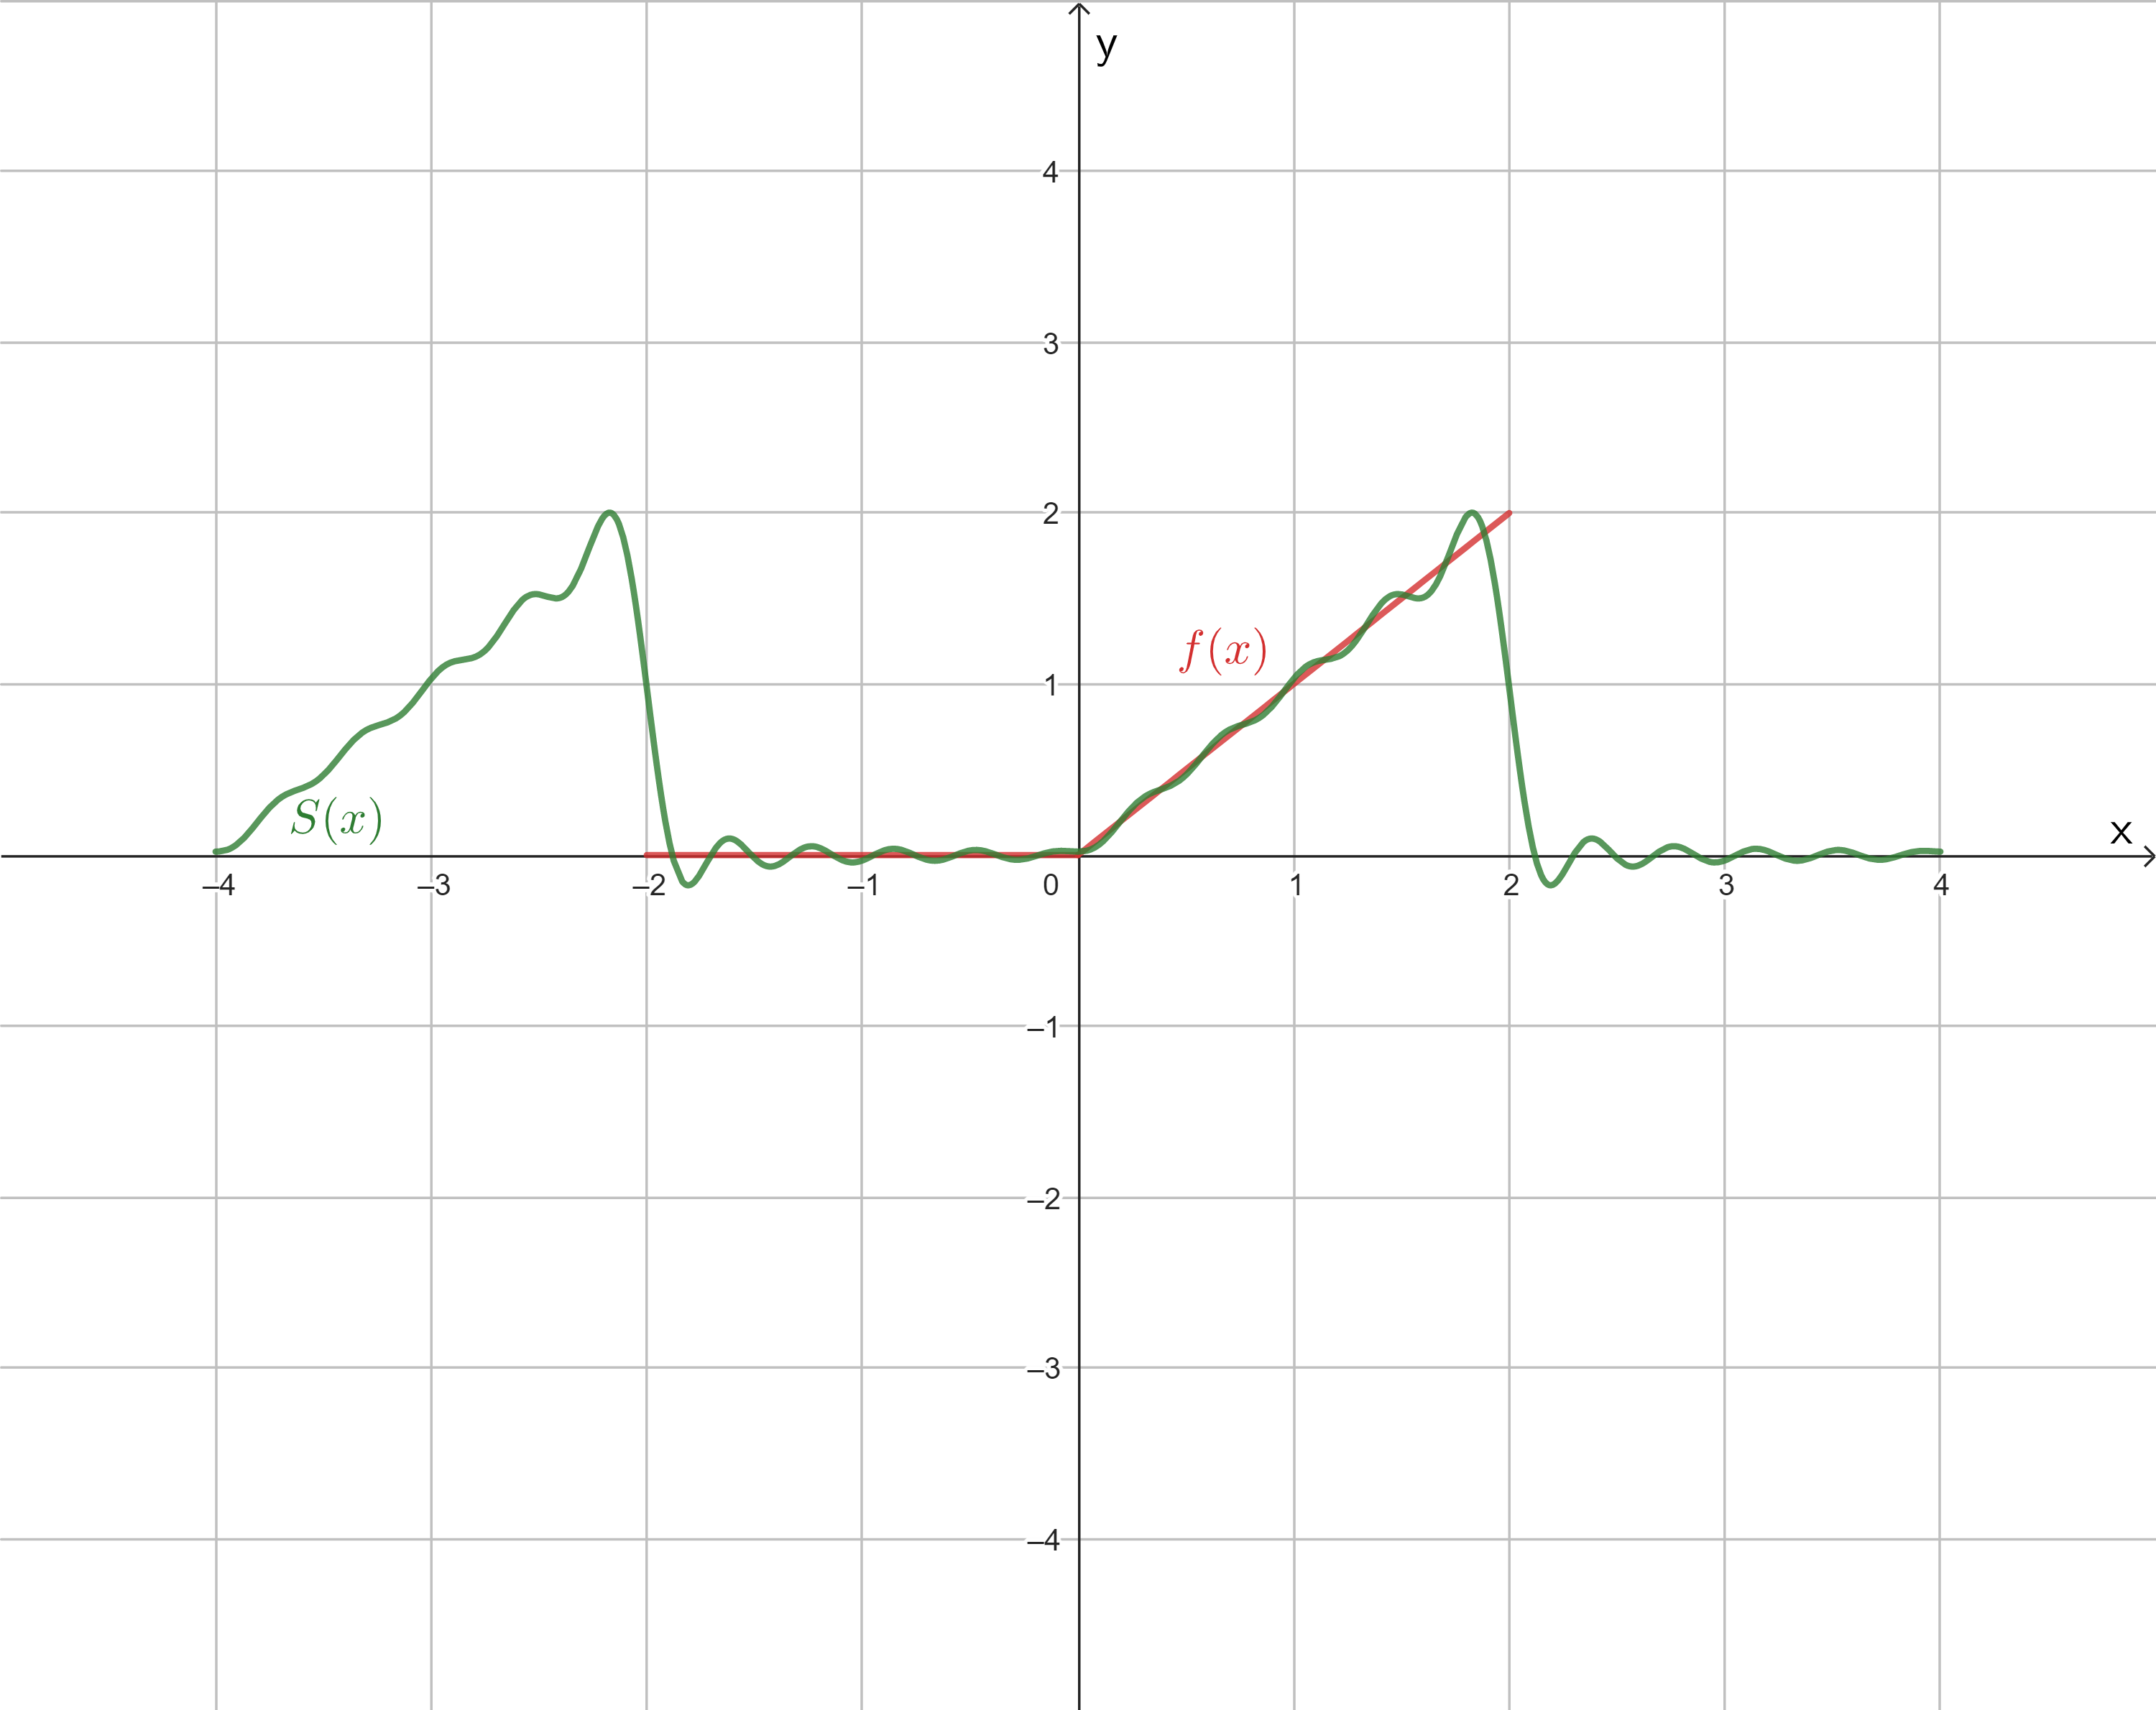
\includegraphics[width=0.43\textwidth]{graph}
\end{figure} \\
Ряд построен верно, т.к. хорошо сходится к исходной функции при $n \rightarrow \infty$.
\end{document}